\begin{appendix}
    \chapter*{Appendices}
    \label{cha:appendices}
    \addcontentsline{toc}{chapter}{Appendices}

    \includeappendixpdfwithtitle{Task Description from Norkart}{appendices/project_description.pdf}{app:task-description}

    % \newgeometry{top=.5in}
    % 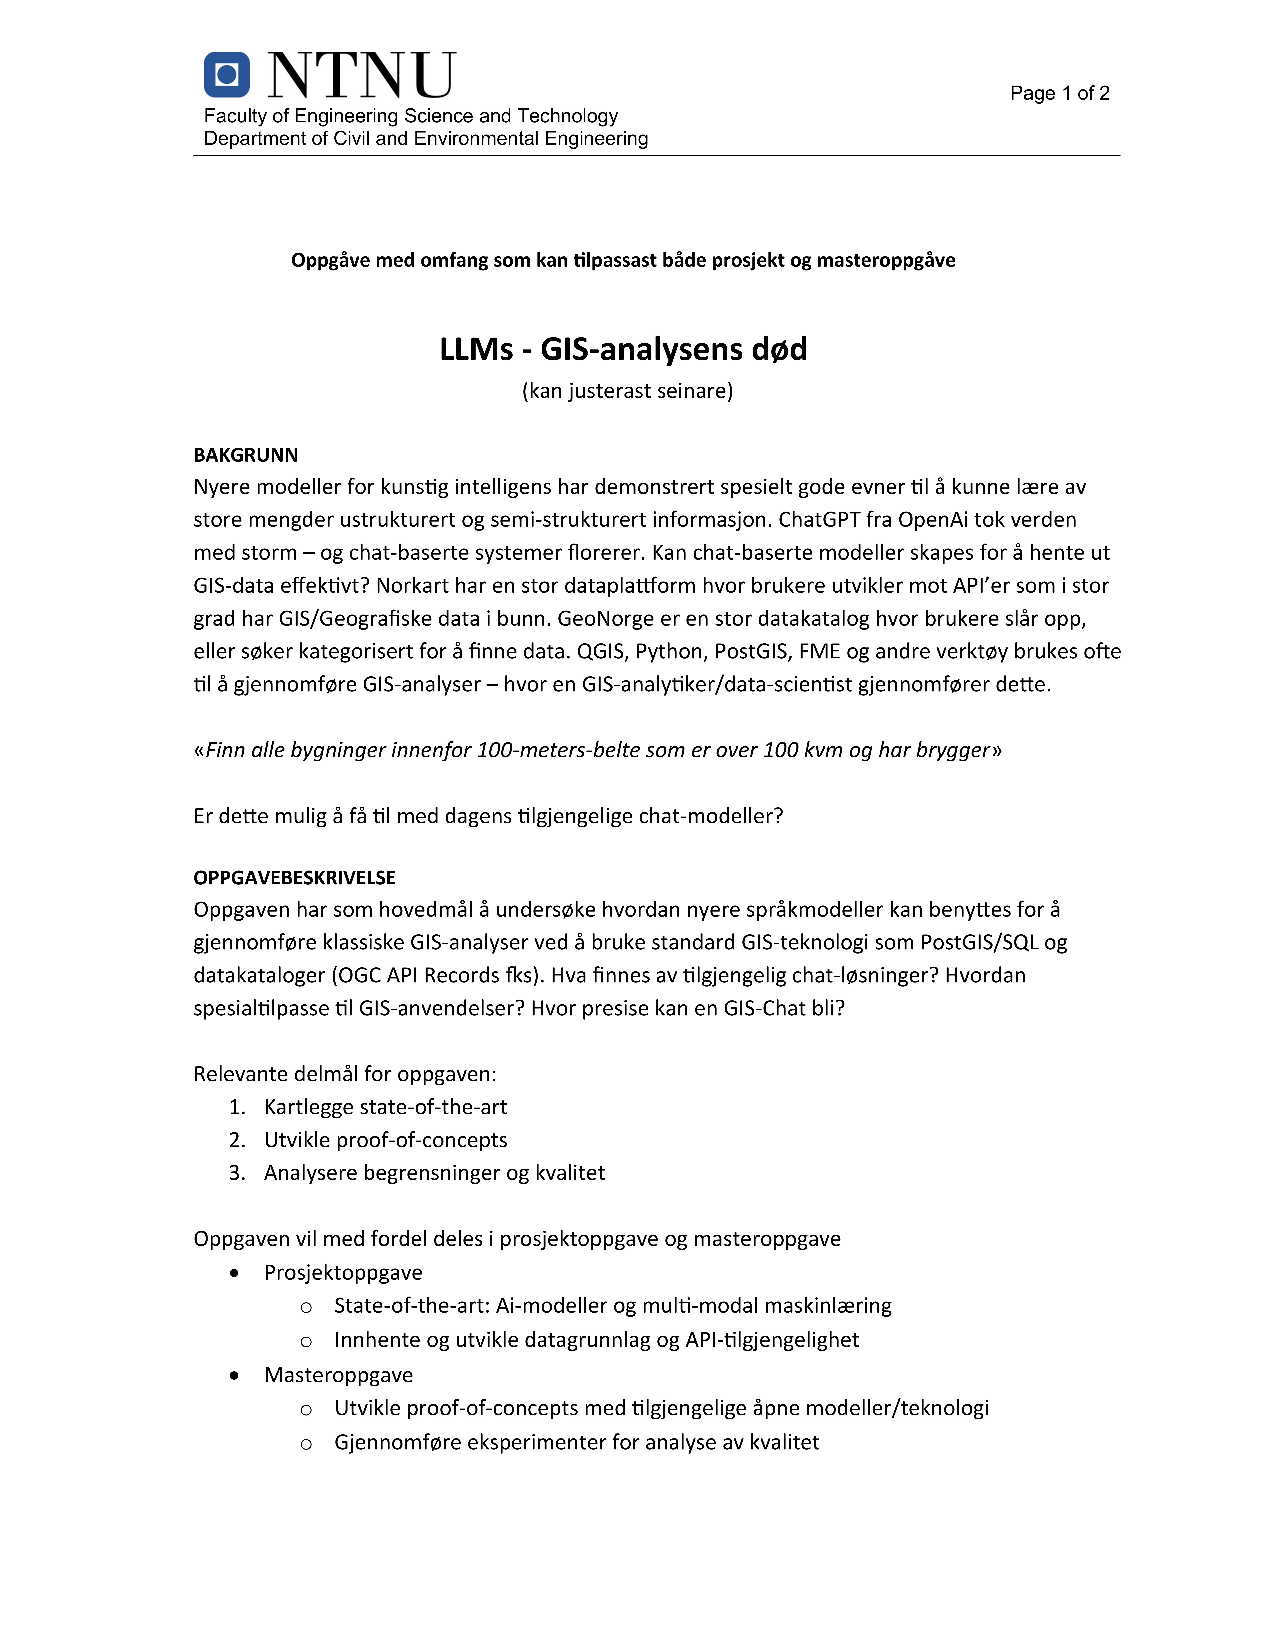
\includepdf[pages=1, scale=.7, pagecommand={\chapter{Task Description from Norkart}\label{app:task-description}}, linktodoc=true]{appendices/project_description.pdf}
    % \restoregeometry
    % \includepdf[pages=2-, scale=.7, pagecommand={}, linktodoc=true]{appendices/project_description.pdf}

    %     \chapter{API Schemas}

    %     \section[OGC API - Features]{\acrshort{acr:ogc} \acrshort{acr:api} - Features}

    %     \acrshort{acr:ogc} \acrshort{acr:api} specification for a 'collection' object\footnote{\url{https://schemas.opengis.net/ogcapi/features/part1/1.0/openapi/schemas/collection.yaml} (retrieved October 25, 2023)}:

    %     \begin{lstlisting}[style=yaml]
    %         type: object
    %         required:
    %         - id
    %         - links
    %         properties:
    %         id:
    %         description: identifier of the collection used, for example, in URIs
    %         type: string
    %         example: address
    %         title:
    %         description: human readable title of the collection
    %         type: string
    %         example: address
    %         description:
    %         description: a description of the features in the collection
    %         type: string
    %         example: An address.
    %         links:
    %         type: array
    %         items:
    %         $ref: link.yaml
    %     example:
    %       - href: http://data.example.com/buildings
    %       rel: item
    %       - href: http://example.com/concepts/buildings.html
    %       rel: describedby
    %         type: text/html
    %   extent:
    %     $ref: extent.yaml
    %   itemType:
    %   description: indicator about the type of the items in the collection (the default value is 'feature').
    %     type: string
    %     default: feature
    %     crs:
    %     description: the list of coordinate reference systems supported by the service
    %     type: array
    %     items:
    %       type: string
    %     default:
    %       - http://www.opengis.net/def/crs/OGC/1.3/CRS84
    %     example:
    %       - http://www.opengis.net/def/crs/OGC/1.3/CRS84
    %       - http://www.opengis.net/def/crs/EPSG/0/4326
    %     \end{lstlisting}

    %     \section[STAC API]{\acrshort{acr:stac} \acrshort{acr:api}}

    %     \chapter{Code Examples}

\end{appendix}